\begin{document}
\extrawidth{0.5in} \extrafootheight{-0in} \pagestyle{headandfoot}
\headrule \header{\textbf{cs2311 - Fall 2014}}{\textbf{HW
 5 \ifprintanswers - Solutions \fi}}{\textbf{Due: Fri. 10/17/14}} \footrule \footer{}{Page \thepage\
of \numpages}{}

\ifprintanswers
% \noindent You should \underline{complete all problems}, but \underline{only a subset will be graded} (which will be graded is not known to you ahead of time). 
\else
\noindent \textbf{Instructions:} All assignments are due \underline{by \textbf{4pm} on the due date} specified.  There will be a box in the CS department office (Rekhi 221) where assignments may be turned in.  Solutions will be posted on-line at the following lecture.  Every student
must write up their own solutions in their own manner.

\medskip
\noindent Please present your solutions in a clean, understandable
manner; pages should be stapled before being turned in, no ragged edges of
paper.

% \medskip
% \noindent Be clear with you penmanship to distinguish set brackets and parentheses.
%   For example, $\{1, 2\}$ is a set where $(1,2)$ is an ordered pair.  Also,
% differentiate the empty set $\emptyset$ and the number zero 0.

\medskip
\noindent You should \underline{complete all problems}, but \underline{only a subset will be graded} (which will be graded is not known to you ahead of time). 
\fi

\begin{questions}

\gquestion{22}{14}{b,d,e,g,i,j,l,m} 
Given the following directed graph showing a relation $R$ of flights between cities.  Answer the following questions.
	\ifprintanswers
	\begin{center}
	    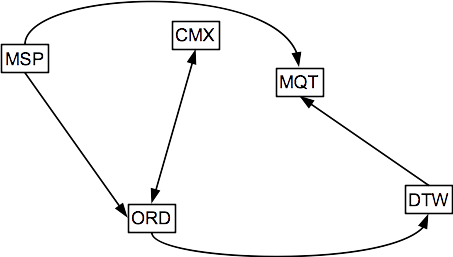
\includegraphics[width=2.2in]{example_relations_f14}
	\end{center}
	\else
	\begin{center}
		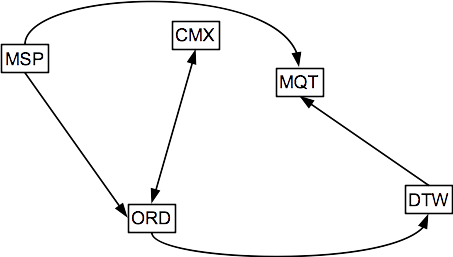
\includegraphics[width=3.5in]{example_relations_f14}
	\end{center}
	\fi

	\ifprintanswers
	\else
	\begin{enumerate}[label=(\alph*),itemsep=0pt,parsep=0pt,topsep=0pt,partopsep=0pt]
		\item (1pt) Give the set $A$ the relation $R$ is on.
		\item (1pt) Give the relation $R$ (that is, list the ordered pairs explicitly).
		\item (2pt) Express the relation $R$ as a zero-one matrix (present cities in alphabetic order, e.g., CMX, DTW, MQT, ...)
		\item (2pt) Find the diagonal relation on $A$ (list all ordered pairs explicitly). 
		\item (2pt) Find the reflexive closure of $R$ (list all ordered pairs explicitly).
		\item (2pt) Find $R^{-1}$ (list all ordered pairs explicitly).
		\item (2pt) Find the symmetric closure of $R$. 
		\item (1pt) Describe what the pairs in $R \circ R$ represent.
		\item (2pt) Find $R \circ R$ (list all ordered pairs explicitly). 
		\item (1pt) Describe what the pairs in $R^3$ represent.
		\item (2pt) Find $R^3$ (list all ordered pairs explicitly).
		\item (1pt) Describe what the transitive closure, $R^{*}$ represents.
		\item (3pt) Find $R^{*}$ (list all ordered pairs explicitly).
	\end{enumerate}
	\fi

    \ifprintanswers
        \vspace{-10pt}
    \fi
    \begin{EnvFullwidth}
    \begin{solution}
    \small
    \begin{enumerate}[label=(\alph*)]
    	\item Give the set $A$ the relation $R$ is on. \\
    	$A = \{ \text{CMX}, \text{DTW}, \text{MQT}, \text{MSP}, \text{ORD} \}$
    	\item Give the relation $R$ (that is, list the ordered pairs explicitly). \\
    	$R = \{ (\CMX, \ORD), (\DTW, \MQT), (\MSP, \MQT), (\MSP, \ORD), (\ORD, \CMX), (\ORD, \DTW) \}$
    	\item Express the relation $R$ as a zero-one matrix \\
    	$R = \begin{bmatrix}
    			0 & 0 & 0 & 0 & 1 \\
    			0 & 0 & 1 & 0 & 0 \\
    			0 & 0 & 0 & 0 & 0 \\
    			0 & 0 & 1 & 0 & 1 \\
    			1 & 1 & 0 & 0 & 0 \\
    			\end{bmatrix} $
    	\item Find the diagonal relation on $A$ (list all ordered pairs explicitly). \\
    	$\Delta = \{ (\CMX, \CMX), (\DTW, \DTW), (\MQT, \MQT), (\MSP, \MSP), (\ORD, \ORD) \}$
    	\item Find the reflexive closure of $R$ (list all ordered pairs explicitly). \\
    	$R \cup \Delta = \{ (\CMX, \ORD), (\DTW, \MQT), (\MSP, \MQT), (\MSP, \ORD), (\ORD, \CMX),$ \\
    	\hspace*{0.4in} $ (\ORD, \DTW), (\CMX, \CMX), (\DTW, \DTW), (\MQT, \MQT), (\MSP, \MSP), (\ORD, \ORD)  \}$
    	\item Find $R^{-1}$ (list all ordered pairs explicitly). \\
    	$R^{-1} = \{ (\ORD, \CMX), (\MQT, \DTW), (\MQT, \MSP), (\ORD, \MSP), (\ORD, \CMX), (\DTW, \ORD) \}$
    	\item Find the symmetric closure of $R$. \\
    	$R \cup R^{-1} = \{ (\CMX, \ORD), (\DTW, \MQT), (\MSP, \MQT), (\MSP, \ORD), (\ORD, \CMX), (\ORD, \DTW), $ \\
    	\hspace*{0.4in} $(\MQT, \DTW), (\MQT, \MSP), (\ORD, \MSP), (\DTW, \ORD) \}$
    	\item Describe what the pairs in $R \circ R$ represent. \\
    	\textit{the cities for which you can travel between in two flights}
    	\item Find $R \circ R$ (list all ordered pairs explicitly). \\
    	$R \circ R = \{ (\CMX, \CMX), (\CMX, \DTW), (\MSP, \CMX), (\MSP, \DTW), (\ORD, \ORD), (\ORD, \MQT) \}$
    	\item Describe what the pairs in $R^3$ represent. \\
    	\textit{the cities for which you can travel between in three flights}
    	\item Find $R^3$ (list all ordered pairs explicitly). \\
    	$R^2 \circ R = \{ (\CMX, \ORD), (\CMX, \MQT), (\MSP, \ORD), (\MSP, \MQT), (\ORD, \CMX), (\ORD, \DTW) \}$ 
    	\item Describe what the transitive closure, $R^{*}$ represents.  \\
    	\textit{the cities for which you can travel between in taking some number of flights}
    	\item Find $R^{*}$ (list all ordered pairs explicitly). \\
    	$R^* = \{ (\CMX, \CMX),  (\CMX, \DTW),  (\CMX, \MQT),  (\CMX, \ORD),  (\DTW, \MQT),  (\MSP, \CMX), $ \\
    	$  (\MSP, \DTW),  (\MSP, \MQT),  (\MSP, \ORD),  (\ORD, \CMX),  (\ORD, \DTW),  (\ORD, \MQT),  (\ORD, \ORD) \} $
    \end{enumerate}
    \end{solution}
    \end{EnvFullwidth}



\gquestion{14}{10}{a-c} Consider the following relations on the sets \textit{Directors} $ = D = \{$\text{Spielberg}, \text{Scorsese}, \text{Bigelow} $\}$, \textit{Movies} $ = M = \{$\text{Saving Private Ryan}, \text{Lincoln}, \text{Catch Me If You Can}, \text{The Departed}, \text{Zero Dark Thirty}, \text{Hurt Locker}  $\}$, \textit{Actors} $= A = \{$\text{Leonardo DiCaprio}, \text{Tom Hanks}, \text{Matt Damon}, \text{Martin Sheen}, \text{Jessica Chastain}, \text{Jeremy Renner} $\}$

Consider the relation $R$ from \textit{Directors} to \textit{Movies} and $S$ from \textit{Movies} to \textit{Actors}.
\begin{align*}
R &= \{ (\text{Spielberg}, \text{Saving Private Ryan}), 
		(\text{Spielberg}, \text{Lincoln}), 
		(\text{Spielberg}, \text{Catch Me If You Can}), \\
  		& \quad  (\text{Scorsese}, \text{The Departed}), 
  		(\text{Bigelow}, \text{Zero Dark Thirty}), 
  		(\text{Bigelow}, \text{Hurt Locker}) \} \\
S &= \{ (\text{Saving Private Ryan}, \text{Tom Hanks}), 
		(\text{Saving Private Ryan}, \text{Matt Damon}),  \\
  		& \quad  (\text{Catch Me If You Can}, \text{Leonardo DiCaprio}), 
  		(\text{Catch Me If You Can}, \text{Martin Sheen}),  \\
  		& \quad (\text{The Departed}, \text{Leonardo DiCaprio}), 
  		(\text{The Departed}, \text{Martin Sheen}),  \\
  		& \quad (\text{Zero Dark Thirty}, \text{Jessica Chastain}), 
  		(\text{Hurt Locker}, \text{Jeremy Renner})  \}
\end{align*}
	\ifprintanswers
	\else
	\begin{enumerate}[label=(\alph*)]
		\item What is $S \circ R$?
		\item Construct $T = S \circ S^{-1}$.
		\item What is $T^*$, describe it in words the relation from $X$ to $Y$ with \ldots
		\item Calculate $T^*$
	\end{enumerate}
	\fi

	\ifprintanswers
        \vspace{-30pt}
    \fi
    \begin{EnvFullwidth}
    \begin{solution}
    \small
    \begin{enumerate}[label=(\alph*)]
    	\item What is $S \circ R$? \\
    	$S \circ R = \{ (\text{Spielberg}, \text{Tom Hanks}), 
    					(\text{Spielberg}, \text{Matt Damon}), 
    					(\text{Spielberg}, \text{Leonardo DiCaprio}), \\
    					(\text{Spielberg}, \text{Martin Sheen}), 
    					(\text{Scorsese}, \text{Leonardo DiCaprio}), 
    					(\text{Scorsese}, \text{Martin Sheen}), \\
    					(\text{Bigelow}, \text{Jessica Chastain}),
    					(\text{Bigelow}, \text{Jeremy Renner})  \}$
    	\item $T = S \circ S^{-1}$ \\
    	$S^{-1} = \{ (\text{Tom Hanks}, \text{Saving Private Ryan}), 
					(\text{Matt Damon}, \text{Saving Private Ryan}),  \\
  			 \quad  (\text{Leonardo DiCaprio}, \text{Catch Me If You Can}), 
  					(\text{Martin Sheen}, \text{Catch Me If You Can}),  \\
  			 \quad (\text{Leonardo DiCaprio}, \text{The Departed}), 
  					(\text{Martin Sheen}, \text{The Departed}),  \\
  			 \quad (\text{Jessica Chastain}, \text{Zero Dark Thirty}), 
  					(\text{Jeremy Renner}, \text{Hurt Locker})  \}$ \\[4pt]
  		$T = S \circ S^{-1} = \{  (\text{Tom Hanks}, \text{Tom Hanks}) 
  					(\text{Matt Damon}, \text{Matt Damon}),  \\
  					(\text{Leonardo DiCaprio}, \text{Leonardo DiCaprio}), 
  					(\text{Martin Sheen}, \text{Martin Sheen}), \\
  					(\text{Jessica Chastain}, \text{Jessica Chastain}), 
  					(\text{Jeremy Renner}, \text{Jeremy Renner}), \\
  					(\text{Tom Hanks}, \text{Matt Damon}), 
  					(\text{Matt Damon}, \text{Tom Hanks}), \\
  					(\text{Leonardo DiCaprio}, \text{Martin Sheen}), 
  					(\text{Martin Sheen}, \text{Leonardo DiCaprio})  \}$
  		\item $T$ is the relation from \textit{Actors} to \textit{Actors} with the first actor appearing in a film with the second.
  		\item  $T^* = \{  (\text{Tom Hanks}, \text{Tom Hanks}) 
  					(\text{Matt Damon}, \text{Matt Damon}) , \\
  					(\text{Leonardo DiCaprio}, \text{Leonardo DiCaprio}), 
  					(\text{Martin Sheen}, \text{Martin Sheen}), \\
  					(\text{Jessica Chastain}, \text{Jessica Chastain}), 
  					(\text{Jeremy Renner}, \text{Jeremy Renner}), \\
  					(\text{Tom Hanks}, \text{Matt Damon}), 
  					(\text{Matt Damon}, \text{Tom Hanks}), \\
  					(\text{Leonardo DiCaprio}, \text{Martin Sheen}), 
  					(\text{Martin Sheen}, \text{Leonardo DiCaprio})  \}$
    \end{enumerate}
    \end{solution}
    \end{EnvFullwidth}



\gquestion{8}{2}{c} Rosen Ch 9.5 \# 2(a,c-e) p. 615
    \ifprintanswers
        \vspace{-15pt}
    \fi
    \begin{EnvFullwidth}
    \begin{solution}
    Which of these relations on the set of all people are equivalence relations?  Determine the properties of an equivalence relation that the others lack. \\
        \begin{tabular}{l}
        (a) $\{(a,b) \;|\; a \;\text{and}\; b \;\text{are the same age}\;\}$. \\
          Equivalence relation \\
%        a) $\{(a,b) \;|\; a \;\text{and}\; b \;\text{are the same age}\;\}$. \\
        % b) $\{(a,b) \;|\; a \;\text{and}\; b \;\text{have the same parents}\;\}$. \\
        % Equivalence relation\\
        
       (c) $\{(a,b) \;|\; a \;\text{and}\; b \;\text{share a common parent}\;\}$. \\ Not an equivalence relation, not transitive \\
       \end{tabular}
       \begin{tabular}{l}
        (d) $\{(a,b) \;|\; a \;\text{and}\; b \;\text{have met}\;\}$. \\
        No, It is not transitive.\\
       (e) $\{(a,b) \;|\; a \;\text{and}\; b \;\text{speak a common language}\;\}$. \\ Not an equivalence relation, not transitive \\
        \end{tabular}
    \end{solution}
    \end{EnvFullwidth}


\gquestion{4}{4}{all} Rosen Ch 9.5 \#26, p. 616
    \ifprintanswers
        \vspace{-10pt}
    \fi
    \begin{solution}
    What are the equivalence classes of the equivalence relations in
    Exercise 1? \\
    Only (a) and (c) are equivalence relations. \\
    For (a), each element is its own equivalence class by itself.\\
    For (c), 1 and 2 form an equivalence class and 0 and 3 form
    another two equivalence classes.
    \end{solution}


% DM with Graph theory, Ch 2.4, p. 62, #14c
\ugquestion{4} List all the equivalence relations on the set $\{a, b, c\}$.  (Show the relation be describing the partition on the set).
    \ifprintanswers
        \vspace{-10pt}
    \fi
    \begin{solution}
    There are five such relations
    \[ \{ \{a\}, \{b\}, \{c\} \}; \{ \{a, b\}, \{c\} \}; \{ \{a, c\}, \{b\} \}; 
        \{ \{b, c\}, \{a\} \};  \{ \{a, b, c\} \} \]
    \end{solution}


\gquestion{6}{4}{a,b} Rosen Ch 9.6 \#2(a,b,d), p. 630.
    \ifprintanswers
        \vspace{-10pt}
    \fi
    \begin{solution}
    \begin{itemize}[itemsep=0pt,parsep=0pt,topsep=0pt,partopsep=0pt]
        \item[(a)] The relation is not reflexive, therefore it is not a parial ordering.  The relation is antisymmetric and transitive.
        \item[(b)] The relation is a partial ordering, it is reflexive, antisymmetric, and transitive.
        \item[(d)] The relation is not transitive, therefore it is not a partial ordering.
    \end{itemize}
    \end{solution}


\gquestion{4}{2}{c} Rosen Ch 9.6 \#4(a,c), p. 630.
    \ifprintanswers
        \vspace{-10pt}
    \fi
    \begin{solution}
    \begin{itemize}[itemsep=0pt,parsep=0pt,topsep=0pt,partopsep=0pt]
        \item[(a)] There should be unequal people of the same height, therefore, the relation is not antisymmetric and $(S, R)$ is not a poset.
        \item[(c)] This is a poset, R is reflexive, antisymmetric, and transitive.
    \end{itemize}
    \end{solution}


\bonusquestion[3] Rosen Ch 9.6 \#32(a-f), p. 631.
    \ifprintanswers
        \vspace{-10pt}
    \fi
    \begin{solution}
    \begin{enumerate}[label=(\alph*),itemsep=0pt,parsep=0pt,topsep=0pt,partopsep=0pt]
        \item maximal elements: $\{ l, m\}$
        \item minimal elements: $\{ a, b, c \}$
        \item there is no greatest element
        \item there is no least element
        \item $\{ k, l, m\}$
        \item $\{ k \}$
    \end{enumerate}
    \end{solution}


% \gquestion{8}{4} List those expressions that are tautologies, contradictions, and contingencies?
% 	\begin{enumerate}[label=(\alph*)]
% 		\item $[(p \vee q) \wedge (p \ra r) \wedge (q \ra r)] \ra r$
% 	\end{enumerate}
%     \ifprintanswers
%         \vspace{-15pt}
%     \fi
%     \begin{solution}
%        Tautology:  (a);
%        Contradiction: (b);
%        Contingency:  (a), (c), (d), (e), (f)
%     \end{solution}


% cs2311-f11, hw2
\gquestion{10}{10}{all} Show the following statement is a tautology without using truth tables. Use the equivalence laws from Table 6-8 (model the solutions in the style of book Examples 6-8, pp. 29-30).  Justify each step with laws.
\begin{center}
    $[(p \vee q) \wedge (p \ra r) \wedge (q \ra r)] \ra r$
\end{center}
    \begin{solution}
    \begin{align*}
      [(p \vee q) &\wedge ((p \ra r) \wedge (q \ra r))] \ra r \\
      &\equiv \neg[(p \vee q) \wedge \neg(p \vee r) \wedge \neg (q \vee r)] \vee r \tag{Table 7, rule 1, x3} \\
      &\equiv [\neg(p \vee q) \vee \neg(\neg(p \vee r) \wedge \neg(q \vee r))] \vee r \tag{DeMorgan's} \\
      & \equiv (\neg p \wedge \neg q) \vee (\neg \neg(p \vee r) \vee \neg \neg(q \vee r)) \vee r \tag{DeMorgan's, x2} \\
      & \equiv (\neg p \wedge \neg q) \vee (p \vee r) \vee (q \vee r) \vee r \tag{Double Negation, x2} \\
      & \equiv (\neg p \wedge \neg q) \vee p \vee q \vee r \vee r \vee r \tag{Commutative} \\
      & \equiv (\neg p \wedge \neg q) \vee p \vee q \vee r \vee r \tag{Idempotent} \\
      & \equiv (\neg p \wedge \neg q) \vee p \vee q \vee r \tag{Idempotent} \\
      & \equiv p \vee (\neg p \wedge \neg q) \vee q \vee r \tag{Commutative} \\
      & \equiv (p \vee \neg p) \wedge (p \vee \neg q) \vee q \vee r \tag{Distributive} \\
      & \equiv (\mathbf{T} \wedge (p \vee \neg q) \vee q \vee r \tag{Negation} \\
      & \equiv (p \vee \neg q) \vee q \vee r \tag{Identity} \\
      & \equiv p \vee (\neg q \vee q) \vee r \tag{Associative} \\
      & \equiv p \vee \mathbf{T} \vee r \tag{Negation} \\
      & \equiv \mathbf{T} \vee r \tag{Domination} \\
      & \equiv \mathbf{T} \tag{Domination}
    \end{align*}

    An alternative solution is:
    \begin{align*}
      [(p \vee q) &\wedge ((p \ra r) \wedge (q \ra r))] \ra r \\
       &\equiv [(p \vee q) \wedge ((p \vee q) \ra r)] \ra r \tag{Table 7, rule 7} \\
       &\equiv [(p \vee q) \wedge (\neg (p \vee q) \vee r)] \ra r \tag{Table 7, rule 1} \\
       &\equiv [((p \vee q) \wedge \neg (p \vee q)) \vee ((p \vee q) \wedge r)] \ra r \tag{Distributive} \\
       &\equiv [\mathbf{F} \vee ((p \vee q) \wedge r)] \ra r \tag{Negation} \\
       & \equiv [((p \vee q) \wedge r) \vee \mathbf{F}] \ra r \tag{Commutative} \\
       & \equiv [((p \vee q) \wedge r)] \ra r \tag{Identity} \\
       & \equiv [(p \vee q) \wedge r] \ra r \tag{drop extra ()} \\
       & \equiv \neg [(p \vee q) \wedge r] \vee r \tag{Table 7, rule 1} \\
       & \equiv  [\neg (p \vee q) \vee \neg r] \vee r \tag{DeMorgans} \\
       & \equiv  \neg (p \vee q) \vee [\neg r \vee r ] \tag{Associative} \\
       & \equiv \neg (p \vee q) \vee [r \vee \neg r] \tag{Communtative} \\
       & \equiv \neg (p \vee q) \vee \mathbf{T} \tag{Negation} \\
       & \equiv \mathbf{T} \tag{Domination} 
    \end{align*}



    \end{solution}


% cs2311-s12, HW1
\gquestion{22}{14}{a,c} Prove the following logical equivalences using the
equivalences from Table 6-8 (model the solutions in the style of
book Examples 6-8, pp. 29-30).  Justify each step with laws.
\begin{enumerate}[label=(\alph*),itemsep=0pt,parsep=0pt,topsep=0pt,partopsep=0pt]
    \item $p \ra (q \vee r) \equiv (p \wedge \neg q) \ra r$
    \item $\neg [ r \vee (q \wedge (\neg r \ra \neg p))] \equiv \neg r \wedge (p \vee \neg q) $
    \item $ [ \neg p \wedge (p \vee q) ] \ra q \equiv \mathbf{T}$
\end{enumerate}
    \begin{solution}
    
    (a)
    \begin{align*}
        p &\ra (q \vee r) \equiv (p \wedge \neg q) \ra r \\
            & \equiv \neg p \vee (q \vee r) \tag{Table 7, rule 1} \\
            & \equiv (\neg p \vee q) \vee r) \tag{Associative} \\
            & \equiv \neg (\neg p \vee q) \ra r \tag{Table 7, rule 1} \\
            & \equiv (\neg \neg p \wedge \neg q) \ra r \tag{DeMorgan's} \\
            & \equiv (p \wedge \neg q) \ra r \tag{Double Negation} 
    \end{align*}
An alternative solution is:
    \begin{align*}
        p &\ra (q \vee r) \equiv (p \wedge \neg q) \ra r \\
        & \equiv (p \ra q) \vee (p \ra r) \tag{Table 7, rule 8} \\
        & \equiv (\neg p \vee q) \vee (\neg p \vee r) \tag{Table 7, rule 1, x2} \\
        & \equiv \neg p \vee q \vee \neg p \vee r \tag{drop parenthesis} \\
        & \equiv \neg p \vee \neg p \vee q \vee r \tag{Communtative} \\
        & \equiv \neg p \vee q \vee r \tag{Idempotent Law} \\
        & \equiv (\neg p \vee q) \vee r \tag{add parenthesis} \\
        & \equiv \neg \neg (\neg p \vee q) \vee r \tag{Double Negation} \\
        & \equiv \neg (\neg \neg p \wedge \neg q) \vee r \tag{DeMorgans} \\
        & \equiv \neg (p \wedge \neg q) \vee r \tag{Doulbe Negation} \\
        & \equiv (p \wedge \neg q) \ra r \tag{Table 7, rule 1}
    \end{align*}

    (b)
    \begin{align*} 
      \neg [ r \vee (q & \wedge (\neg r \ra \neg p))] \equiv \neg r \wedge (p \vee \neg q) \\
        & \equiv \neg [r \vee (q \wedge (p \ra r))] \tag{Table 7, rule 2} \\
        & \equiv \neg [r \vee (q \wedge (\neg p \vee r))] \tag{Table 7, rule 1} \\
        & \equiv \neg [r \vee (q \wedge \neg p) \vee (q \wedge r)] \tag{Distributive} \\
        & \equiv \neg [r \vee (q \wedge r) \vee (q \wedge \neg p)] \tag{Commutative} \\
        & \equiv \neg [r \vee (q \wedge \neg p)] \tag{Absorption} \\
        & \equiv \neg [r \vee (\neg p \wedge q)] \tag{Commutative} \\
        & \equiv \neg r \wedge \neg (\neg p \wedge q) \tag{DeMorgan's} \\
        & \equiv \neg r \wedge (\neg \neg p \vee \neg q) \tag{DeMorgan's} \\
        & \equiv \neg r \wedge (p \vee \neg q) \tag{Double Negation} 
    \end{align*}
An alternative solution is:
    \begin{align*} 
      \neg [ r \vee (q & \wedge (\neg r \ra \neg p))] \equiv \neg r \wedge (p \vee \neg q) \\
      & \equiv [\neg r \wedge \neg (q  \wedge (\neg r \ra \neg p))] \tag{DeMorgans} \\
      & \equiv [\neg r \wedge (\neg q \vee \neg (\neg r \ra \neg p))] \tag{DeMorgans} \\
      & \equiv [\neg r \wedge (\neg q \vee (\neg r \wedge \neg \neg p))] \tag{Table 7, rule 5} \\
      & \equiv [\neg r \wedge (\neg q \vee (\neg r \wedge p))] \tag{Double Negation} \\
      & \equiv [\neg r \wedge ((\neg q \vee \neg r) \wedge (\neg q \vee p))] \tag{Distributive} \\
      & \equiv [(\neg r \wedge (\neg q \vee \neg r)) \wedge (\neg q \vee p)] \tag{Associative} \\
      & \equiv [(\neg r \wedge (\neg r \vee \neg q)) \wedge (\neg q \vee p)] \tag{Commutative} \\
      & \equiv [\neg r \wedge (\neg q \vee p)] \tag{Absoption} \\
      & \equiv [\neg r \wedge (p \vee \neg q)] \tag{Commutative} \\
      & \equiv \neg r \wedge (p \vee \neg q) \tag{drop extra ()}
    \end{align*}

    (c)
    There are many possible solutions; two are given.
	\small
    \begin{align*}
        [ \neg p & \wedge (p \vee q) ] \ra q \\
        & \equiv \neg [ \neg p \wedge (p \vee q) ] \vee q \tag{Table 7, rule 1} \\
        & \equiv \neg \neg p \vee \neg (p \vee q) \vee q \tag{DeMorgan's law} \\
        & \equiv p \vee \neg (p \vee q) \vee q \tag{Double Negation} \\
        & \equiv p \vee q \vee \neg (p \vee q) \tag{Commutative} \\
        & \equiv (p \vee q) \vee \neg (p \vee q) \tag{add in parenthesis}\\
        & \equiv \mathbf{T} \tag{Negation} 
    \end{align*}

    \begin{align*}
        [ \neg p & \wedge (p \vee q) ] \ra q \\
        & \equiv \neg [ \neg p \wedge (p \vee q) ] \vee q \tag{Table 7, rule 1} \\
        & \equiv \neg \neg p \vee \neg (p \vee q) \vee q \tag{DeMorgan's law} \\
        & \equiv p \vee \neg (p \vee q) \vee q \tag{Double Negation} \\
        & \equiv p \vee q \vee \neg (p \vee q) \tag{Commutative} \\
        & \equiv p \vee q \vee (\neg p \wedge \neg q) \tag{DeMorgan's} \\
        & \equiv p \vee (q \vee \neg p) \wedge (q \vee \neg q) \tag{Distributive} \\
        & \equiv p \vee (q \vee \neg p) \wedge \mathbf{T} \tag{Negation} \\
        & \equiv p \vee (q \vee \neg p) \tag{Identity} \\
        & \equiv p \vee (\neg p \vee q) \tag{Commutative} \\
        & \equiv (p \vee \neg p) \vee q \tag{Associative} \\
        & \equiv \mathbf{T} \vee q \tag{Negation} \\
        & \equiv \mathbf{T} \tag{Domination}
    \end{align*}
    \end{solution}

\end{questions}
\end{document}